\documentclass[11pt]{report}
\usepackage[utf8]{inputenc}
\usepackage[shortlabels]{enumitem}
\usepackage{cite}
\usepackage{graphicx}
\usepackage{amsmath}
\usepackage{esint}
\usepackage{units}
\usepackage{siunitx}
\usepackage{parskip}
\usepackage{mdframed}
\usepackage{amssymb}
\usepackage{commath}
\usepackage{subfig}
\usepackage{float}
\usepackage[hidelinks]{hyperref}
\usepackage[top=2.54cm, bottom=2.54cm]{geometry}

\sisetup{
	per-mode=fraction,
	fraction-function=\tfrac
}

\hypersetup{
	colorlinks=true,
	linkcolor=blue,
	urlcolor=blue
}

\title{Minimum Notes for AP Physics C: E\&M\\
	\large A lot of invisible stuff, huh?}
\author{Martin Gong / Nanami Kyosuke} 
\date{March 29, 2022\\1st Revision}

\begin{document}
	\maketitle

	\tableofcontents

	\chapter*{Foreword}
\addcontentsline{toc}{chapter}{Foreword}

I wish to jot down my own interpretations of this truly splendid piece of text. The concept of suicide is one that I have struggled with, and with a cursory first read, this book had provided me with a lot of answers to that question.

This set of notes will be written in the form of quotes + annotation. To say the least, it functions partially in the form of annotation for the book \textit{The Myth of Sisyphus}, which, since I have not mentioned, is a book that I recommend everyone to have a read; if you haven't already, you are missing out.

\begin{flushright}
    Martin Weiqi Gong\\
    June 26, 2022
\end{flushright}
	
	\chapter{Coulomb's Law \& Electric Charges}

Coulomb described the interaction between charges, most readily applicable in point charges with the following relation

\[\vec{F} = k \frac{Q_1 Q_2}{r^2} \hat{r} = \frac{1}{4\pi\epsilon_0} \frac{Q_1 Q_2}{r^2} \hat{r}\]

The forces acting on different charges follows the rule of superposition, which means multiple external charges create electrostatic interaction (forces) 

	\chapter{Electric Fields \& Gauss's Law}

\[\Phi_E = \oiint_S \vec{E}\cdot\mathrm{d}\vec{A} = \frac{Q_{\mathrm{enc}}}{\epsilon_0}\]


	
	\chapter{Electric Potential}
	
Just like how we have potential energy in mechanics, we have potential energy in electromagnetism.

	\chapter{DC Circuits}

A circuit is a closed loop in which electricity can ``flow'' through. An open circuit does not allow for any flow.

As it seems, the most important thing about DC circuits at this stage is analyzing them - mostly three important variables: voltage, resistance, and current, with the addition of their change over time.

\section{Resistors (\texorpdfstring{$R$}{R})}

Resistors are elements, or resistance as a property of elements inside a circuit, is something that resists 

\section{Current (\texorpdfstring{$I$}{I})}

\section{EMF (\texorpdfstring{$\mathcal{E}$}{E})}

EMF is an element that provides an electromotive force -- this is measured in Volts. The simple statement is ``EMFs are devices that provide a potential difference of some voltage.'' I do not want to get into the details because it is a complicated concept that can be easily misunderstood, at least for me.

Test for changes.

\section{Circuit \& Circuit Laws}

	\chapter{Capacitance}

A capacitor ``is a device that stores energy in an electrostatic field.'' Capacitors, in general, are made of two metal sheets separated by a dielectric and wrapped in a cylinder. In fact, any two conductive elements not in contact can form a capacitor. When we create a potential difference across these two elements, charges will move from high potential to low potential. With this behavior, capacitors can be seen as a conductor in a circuit that can also be used to store energy. At any instance in time, there are equal amount of charges (positive or the two plates (conductive elements) of the capacitor, given a neutral capacitor and a circuit context. The accumulation of charge is charging the capacitor; vice versa, the charge/energy stored can also be discharged.

Real world capacitors have internal resistance, theoretically modelled capacitors, however, are ideal and do not have resistance. Thus, we consider RC (Resistor, Capacitor) circuits instead of circuits with only the emf and capacitor (this will theoretically cause the capacitor to charge up instantly with infinite current).

Capacitance is first modelled by the relation

\[Q = CV\]

where C is the capacitance measured in \textbf{farads}, Q is the amount of charge to fully charge the capacitor, and V is the voltage given across the capacitor.

Consider the following circuit

\begin{center}
    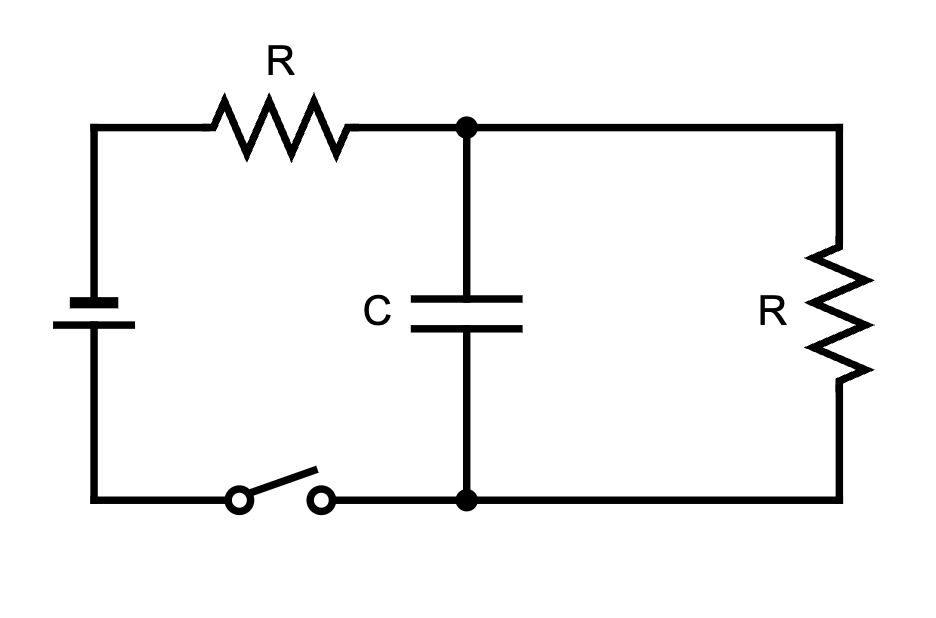
\includegraphics[scale=0.35]{assets/rc-circuit}
\end{center}

We have a switch to break the emf from the circuit, capacitor, and two resistors. 

\section{Charging the Capacitor}

Applying Kirchhoff's Law on the left loop with the switch closed, we obtain 

\begin{align*}
    \mathcal{E} - V_C - IR &= 0\\
    \mathcal{E} - \frac{Q}{C} &= \frac{\mathrm{d}Q}{\mathrm{d}t} R\\
    \int \frac{\mathrm{d}t}{R} &= \int \frac{\mathrm{d}Q}{\mathcal{E} - \frac{Q}{C}}\\
    \frac{t}{R} + C_1 &= -C \ln\abs{\mathcal{E} - \frac{Q}{C}}\\
    -\frac{t}{RC} + C_1 &= \ln\abs{\mathcal{E} - \frac{Q}{C}}\\
    Ae^{-\frac{t}{RC}} &= \mathcal{E} - \frac{Q}{C}\\
    Q(t) &= C \left(\mathcal{E} - Ae^{-\frac{t}{RC}}\right)
\end{align*}

we apply the fact that the capacitor is uncharged at $t = 0$

\[\boxed{Q(t) = C \mathcal{E} \left(1 - e^{-\frac{t}{RC}}\right)}\]

Taking the derivative yields the function of current over time, which is also exponential

\begin{align*}
    Q'(t) = I(t) &= \frac{\mathrm{d}}{\mathrm{d}t} C \mathcal{E} \left(1 - e^{-\frac{t}{RC}}\right)\\
    &= \boxed{\frac{\mathcal{E}}{R} e^{-\frac{t}{RC}}}
\end{align*}

Here's a graph from \href{http://hyperphysics.phy-astr.gsu.edu/hbase/hph.html}{Hyper Physics}

\begin{center}
    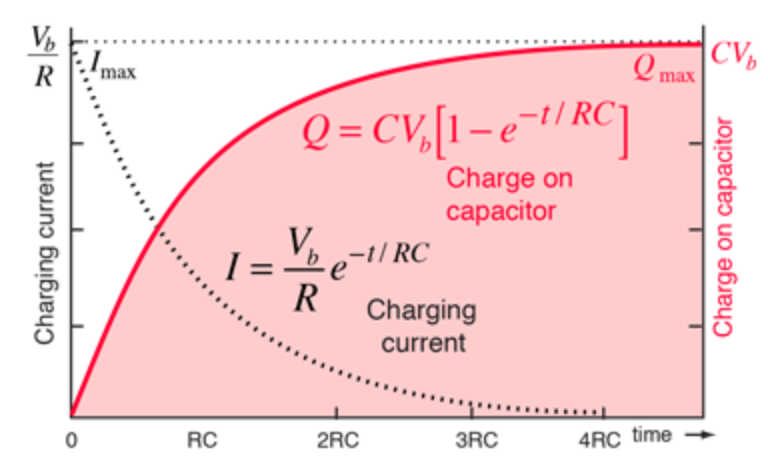
\includegraphics[scale=0.6]{assets/hp-c-charging.png}
\end{center}

\section{Discharging the Capacitor}

Applying Kirchhoff's Law on the right loop (and with some substitution), we obtain 

\begin{align*}
    V_C - IR &= 0\\
    \frac{Q}{C} &= \frac{-\mathrm{d}Q}{\mathrm{d}t} R\\
    -\frac{\mathrm{d}t}{RC} &= \frac{\mathrm{d}Q}{Q}\\
    -\frac{t}{RC} + C_1 &= \ln\abs{Q}\\
    Q(t) &= C_1 e^{-\frac{t}{RC}}\\
    &= Q_0 e^{-\frac{t}{RC}}\\
    &= \boxed{CV_0 e^{-\frac{t}{RC}}}
\end{align*}

Not that $I$ is $-\nicefrac{\mathrm{d}Q}{\mathrm{d}t}$ but not $\nicefrac{\mathrm{d}Q}{\mathrm{d}t}$ because, as the capacitor is discharging, the current is positive on the resistor; change of charge on the capacitor $\mathrm{d}Q_c$, however, is negative. We need to, thus, govern that relationship.

Here's a graph from \href{http://hyperphysics.phy-astr.gsu.edu/hbase/hph.html}{Hyper Physics}

\begin{center}
    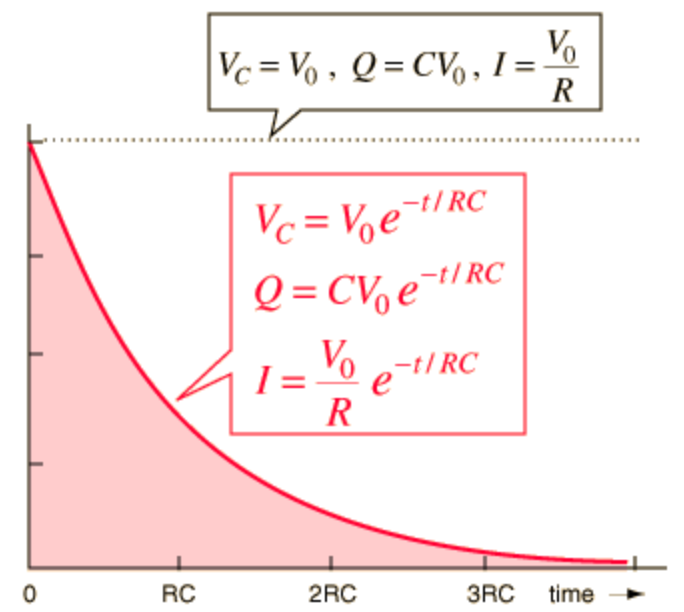
\includegraphics[scale=0.6]{assets/hp-c-discharging.png}
\end{center}

\section{RC Time Constant}

In the exponential functions derived above, we see the the common existence of the $RC$ expression; this is called the \textbf{RC Time Constant}. In general, there is a $63.2\%$ change at $t = RC$, a $86.5\%$ change at $t = 2RC$, and a $95.0\%$ change at $t = 3RC$.

Considering the numerical value of the time constant: the greater $RC$ is, the longer it takes for the capacitor to charge up or discharge.

\section{Energy}

There are many ways to find energy stored by a capacitor, there are, for example, two ways that I know of:
\begin{enumerate}[1.]
    \item By utilizing the relation $P = IV = I^2R$ to sum the power over time, which is energy, of some resistor in an RC circuit.
    \item By summing up the energy of moving all the charges for a capacitor.
\end{enumerate}

For the first method:

\begin{align*}
    U = W &= \int P \,\mathrm{d}t\\
    &= \int I^2R \,\mathrm{d}t\\
    &= \int_0^\infty \left(\frac{V_0}{R} e^{-\frac{t}{RC}}\right)^2 R \,\mathrm{d}t\\
    &= \left.-\frac{1}{2} C{V_0}^2 e^{-\frac{2t}{RC}}\right\vert_0^\infty\\
    &= \boxed{\frac{1}{2} C{V_0}^2 = \frac{1}{2} \frac{Q^2}{C} = \frac{1}{2}QV_0}\\
\end{align*}

For the second method we can see this as moving charge across a certain potential (given by the amount of charge on the plates). The work done will then be

\[\mathrm{d}W = V(q) \mathrm{d}q\]

The total work to move all the charges:

\begin{align*}
    U  = W &= \int_0^Q V(q) \,\mathrm{d}q\\
    &= \int_0^Q \frac{q}{C} \,\mathrm{d}q\\
    &= \boxed{\frac{1}{2} \frac{Q^2}{C} = \frac{1}{2}CV^2 = \frac{1}{2}QV}
\end{align*}

\section{Finding Capacitance}

We know a relation of capacitance

\[Q = CV\]



\section{Dielectric and the Dielectric Constant}

When we add some dielectric between the plates of the capacitor, the electron of the atoms of the dielectric will be at an offset caused by the electrical field of the plates. In other words, they are \textit{polarizable}. This creates an opposing electric field to those created by the plates. Thus, to maintain the same voltage across the plates (to the emf), the charge density of the plates have to increase, causing more charge to be on the capacitor. This directly affects the capacitance and is measured by the \textbf{dielectric constant}, also called \textbf{relative permittivity}: $\kappa$

\[\kappa = \frac{\varepsilon}{\varepsilon_0}\]

where $\varepsilon$ is the permittivity of the material/dielectric, and $\varepsilon_0$ is the permittivity of vacuum.

Capacitance can be found with

\[C = \kappa C_0\]

where $C$ is the capacitance of the capacitor with dielectric, and $C_0$ is the capacitance of capacitor with vacuum.

\section{Capacitor Circuits}

\subsection{Series}

\hfil 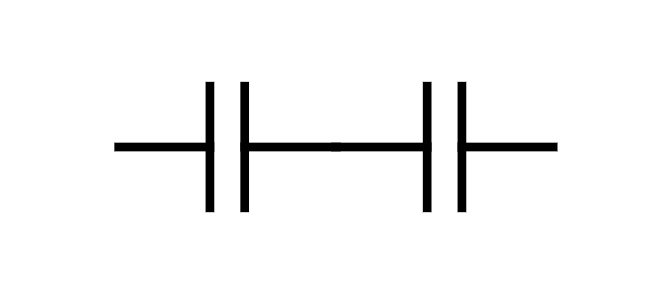
\includegraphics[scale=0.35]{assets/c-series.png}

\subsection{Parallel}

\hfil 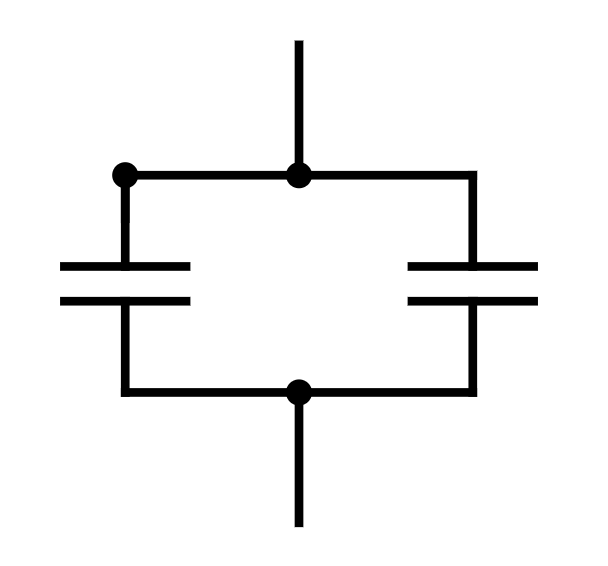
\includegraphics[scale=0.35]{assets/c-parallel.png}

	\chapter{Magnetism}

Magnets (objects that produce magnetic fields) 

Moving charge (current or moving charges) produce magnetic fields and magnetic fields can only be produced by currents similar to how charges produce electric fields and electric fields can only be produced by charges. It is important to note that even in permanent magnets where there is seemingly not charges moving, the magnetic field is still provided by moving charges (provided by the electron spins of well aligned molecules in this case). Magnetic fields exert forces on currents similar to how electric fields exert forces on charges.

\section{Notation}

Note that $\otimes$ (or $\times$) represents current flowing into the page and $\odot$ represents current flowing out of the page. $\vec{B}$ is used to denote the magnetic field.

\section{Interactions}

\subsection{Laws}

Magnetic fields are similar to other fields where the resultant field at some point in space can be written as the vector sum of all magnetic fields at that point. In other words, magnetic fields follow superposition.

Magnetic fields created by currents/moving charges come in loops perpendicular to the direction of current/moving charge and can be memorized with the right hand rule (shown below).

\hfil 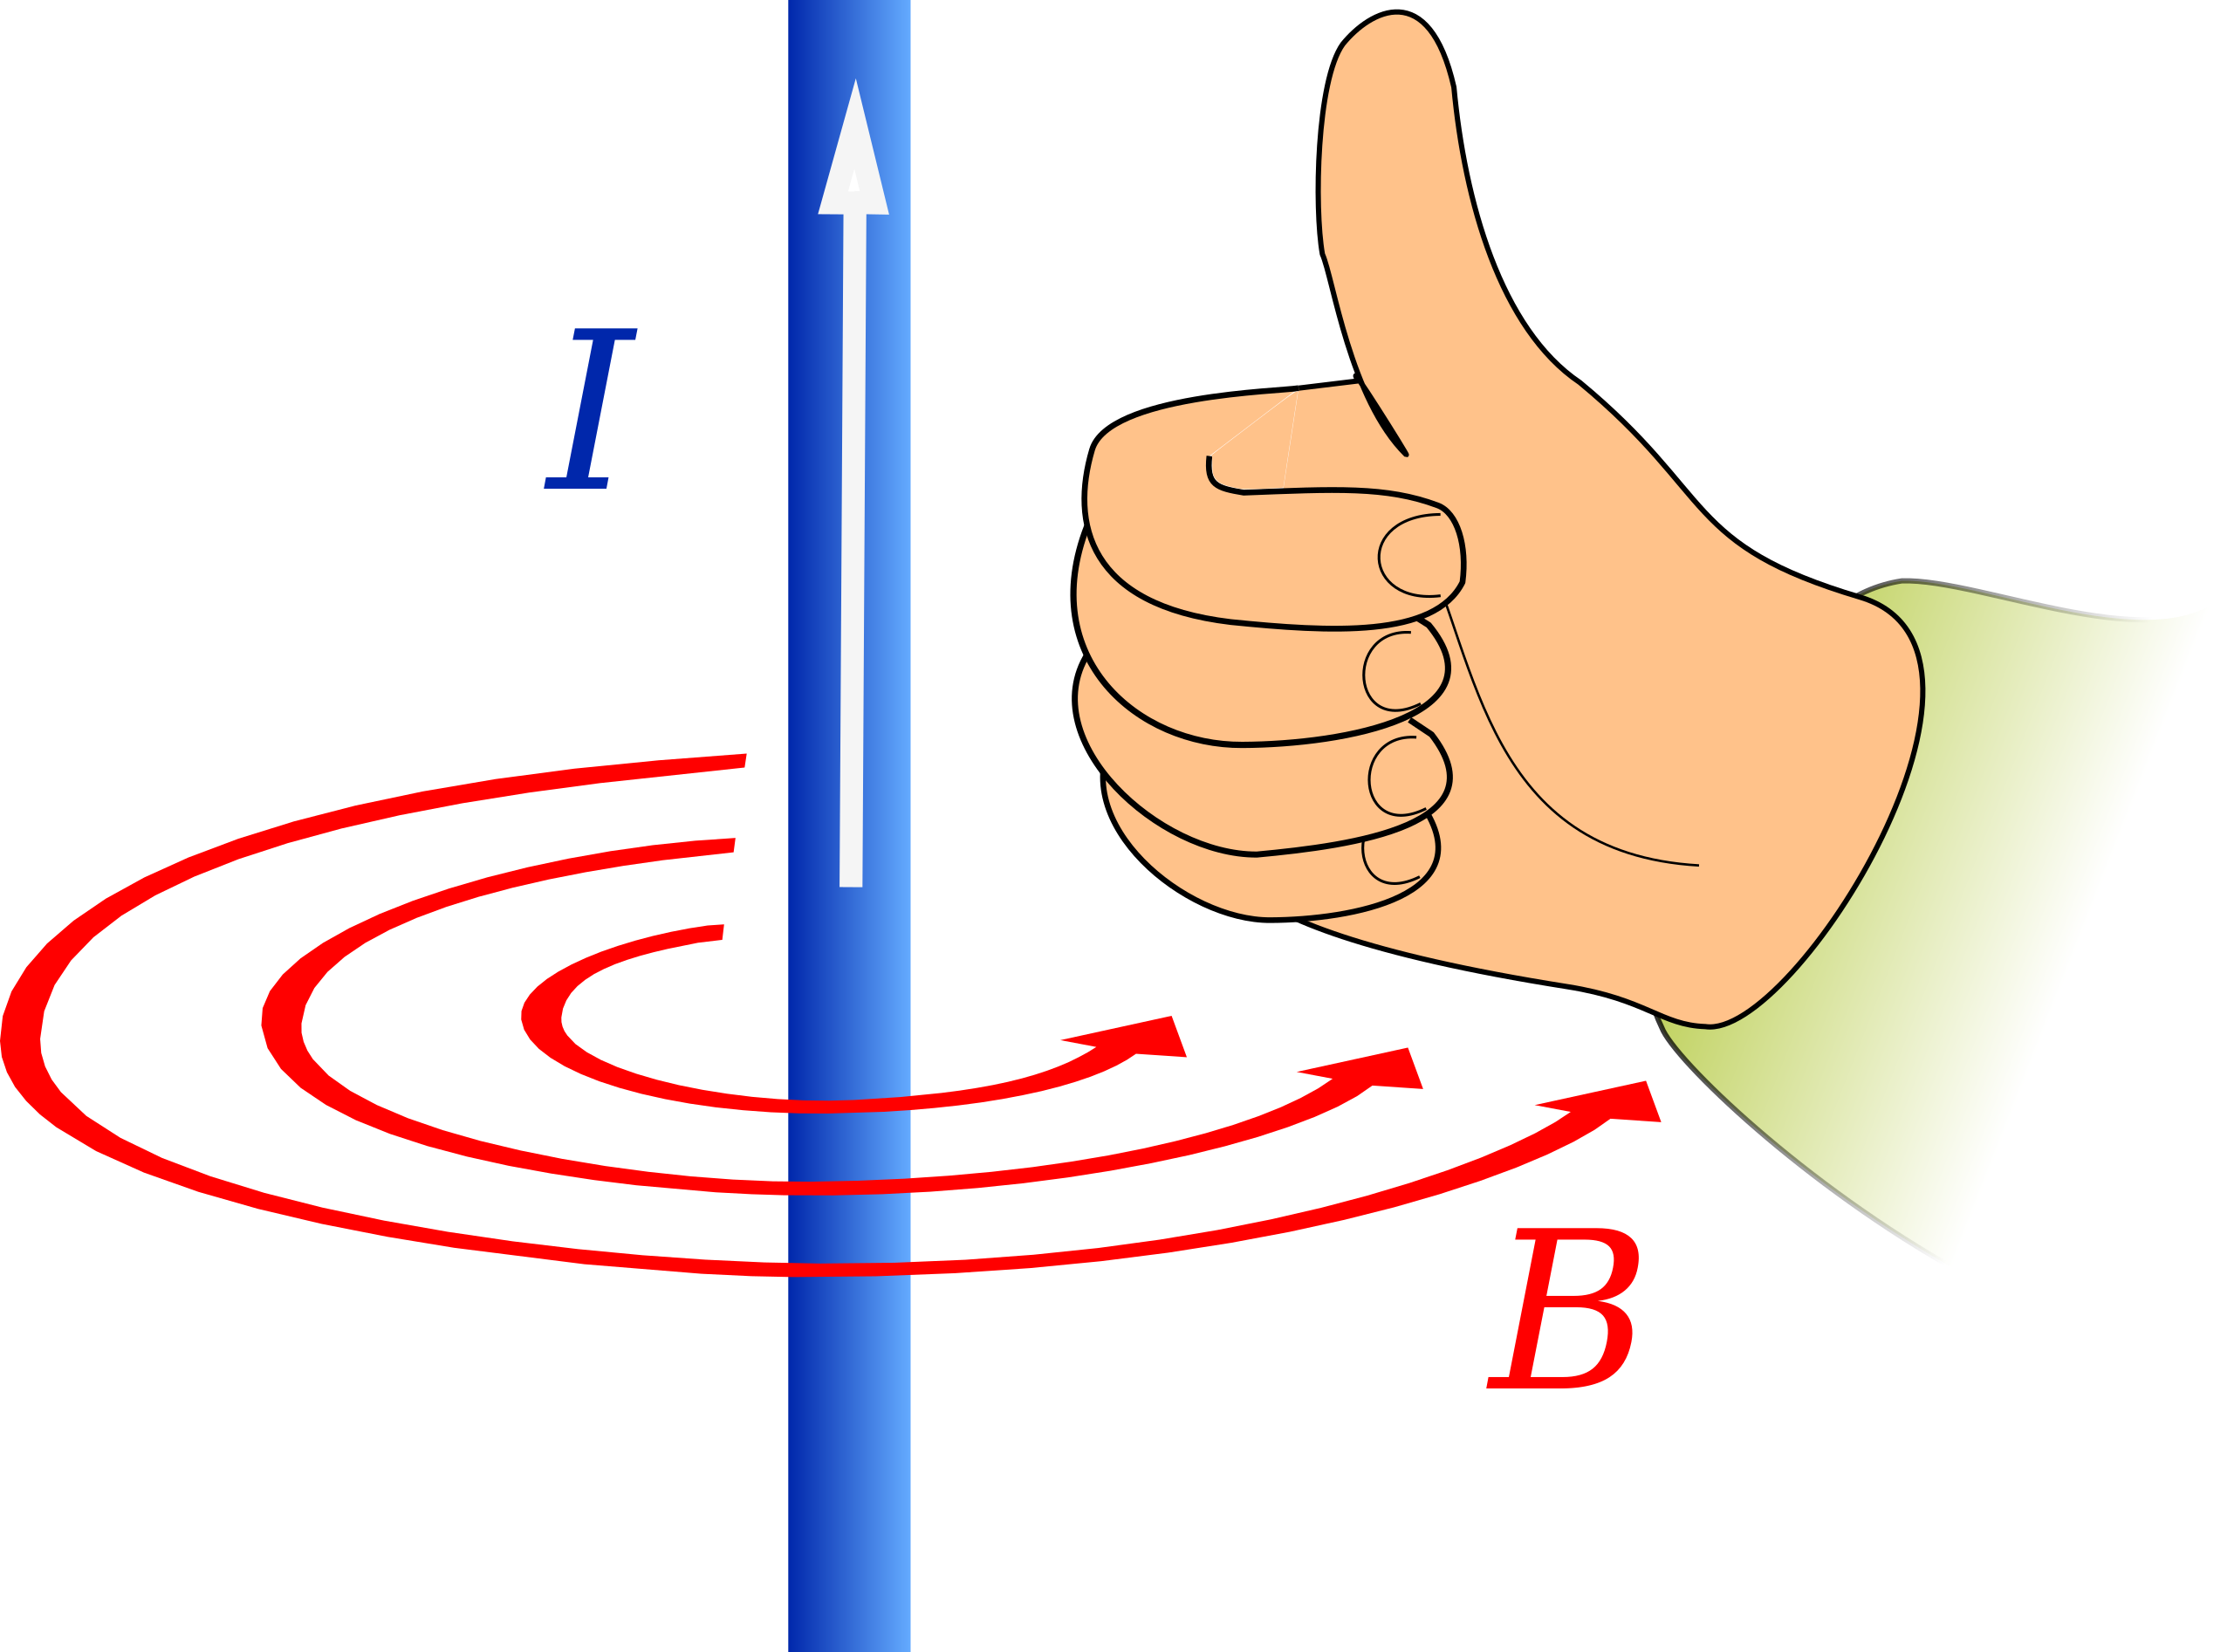
\includegraphics[scale=0.05]{assets/current-rhr.png}

Magnets form magnetic fields with loops coming out of the north pole and going into the south pole.

\hfil 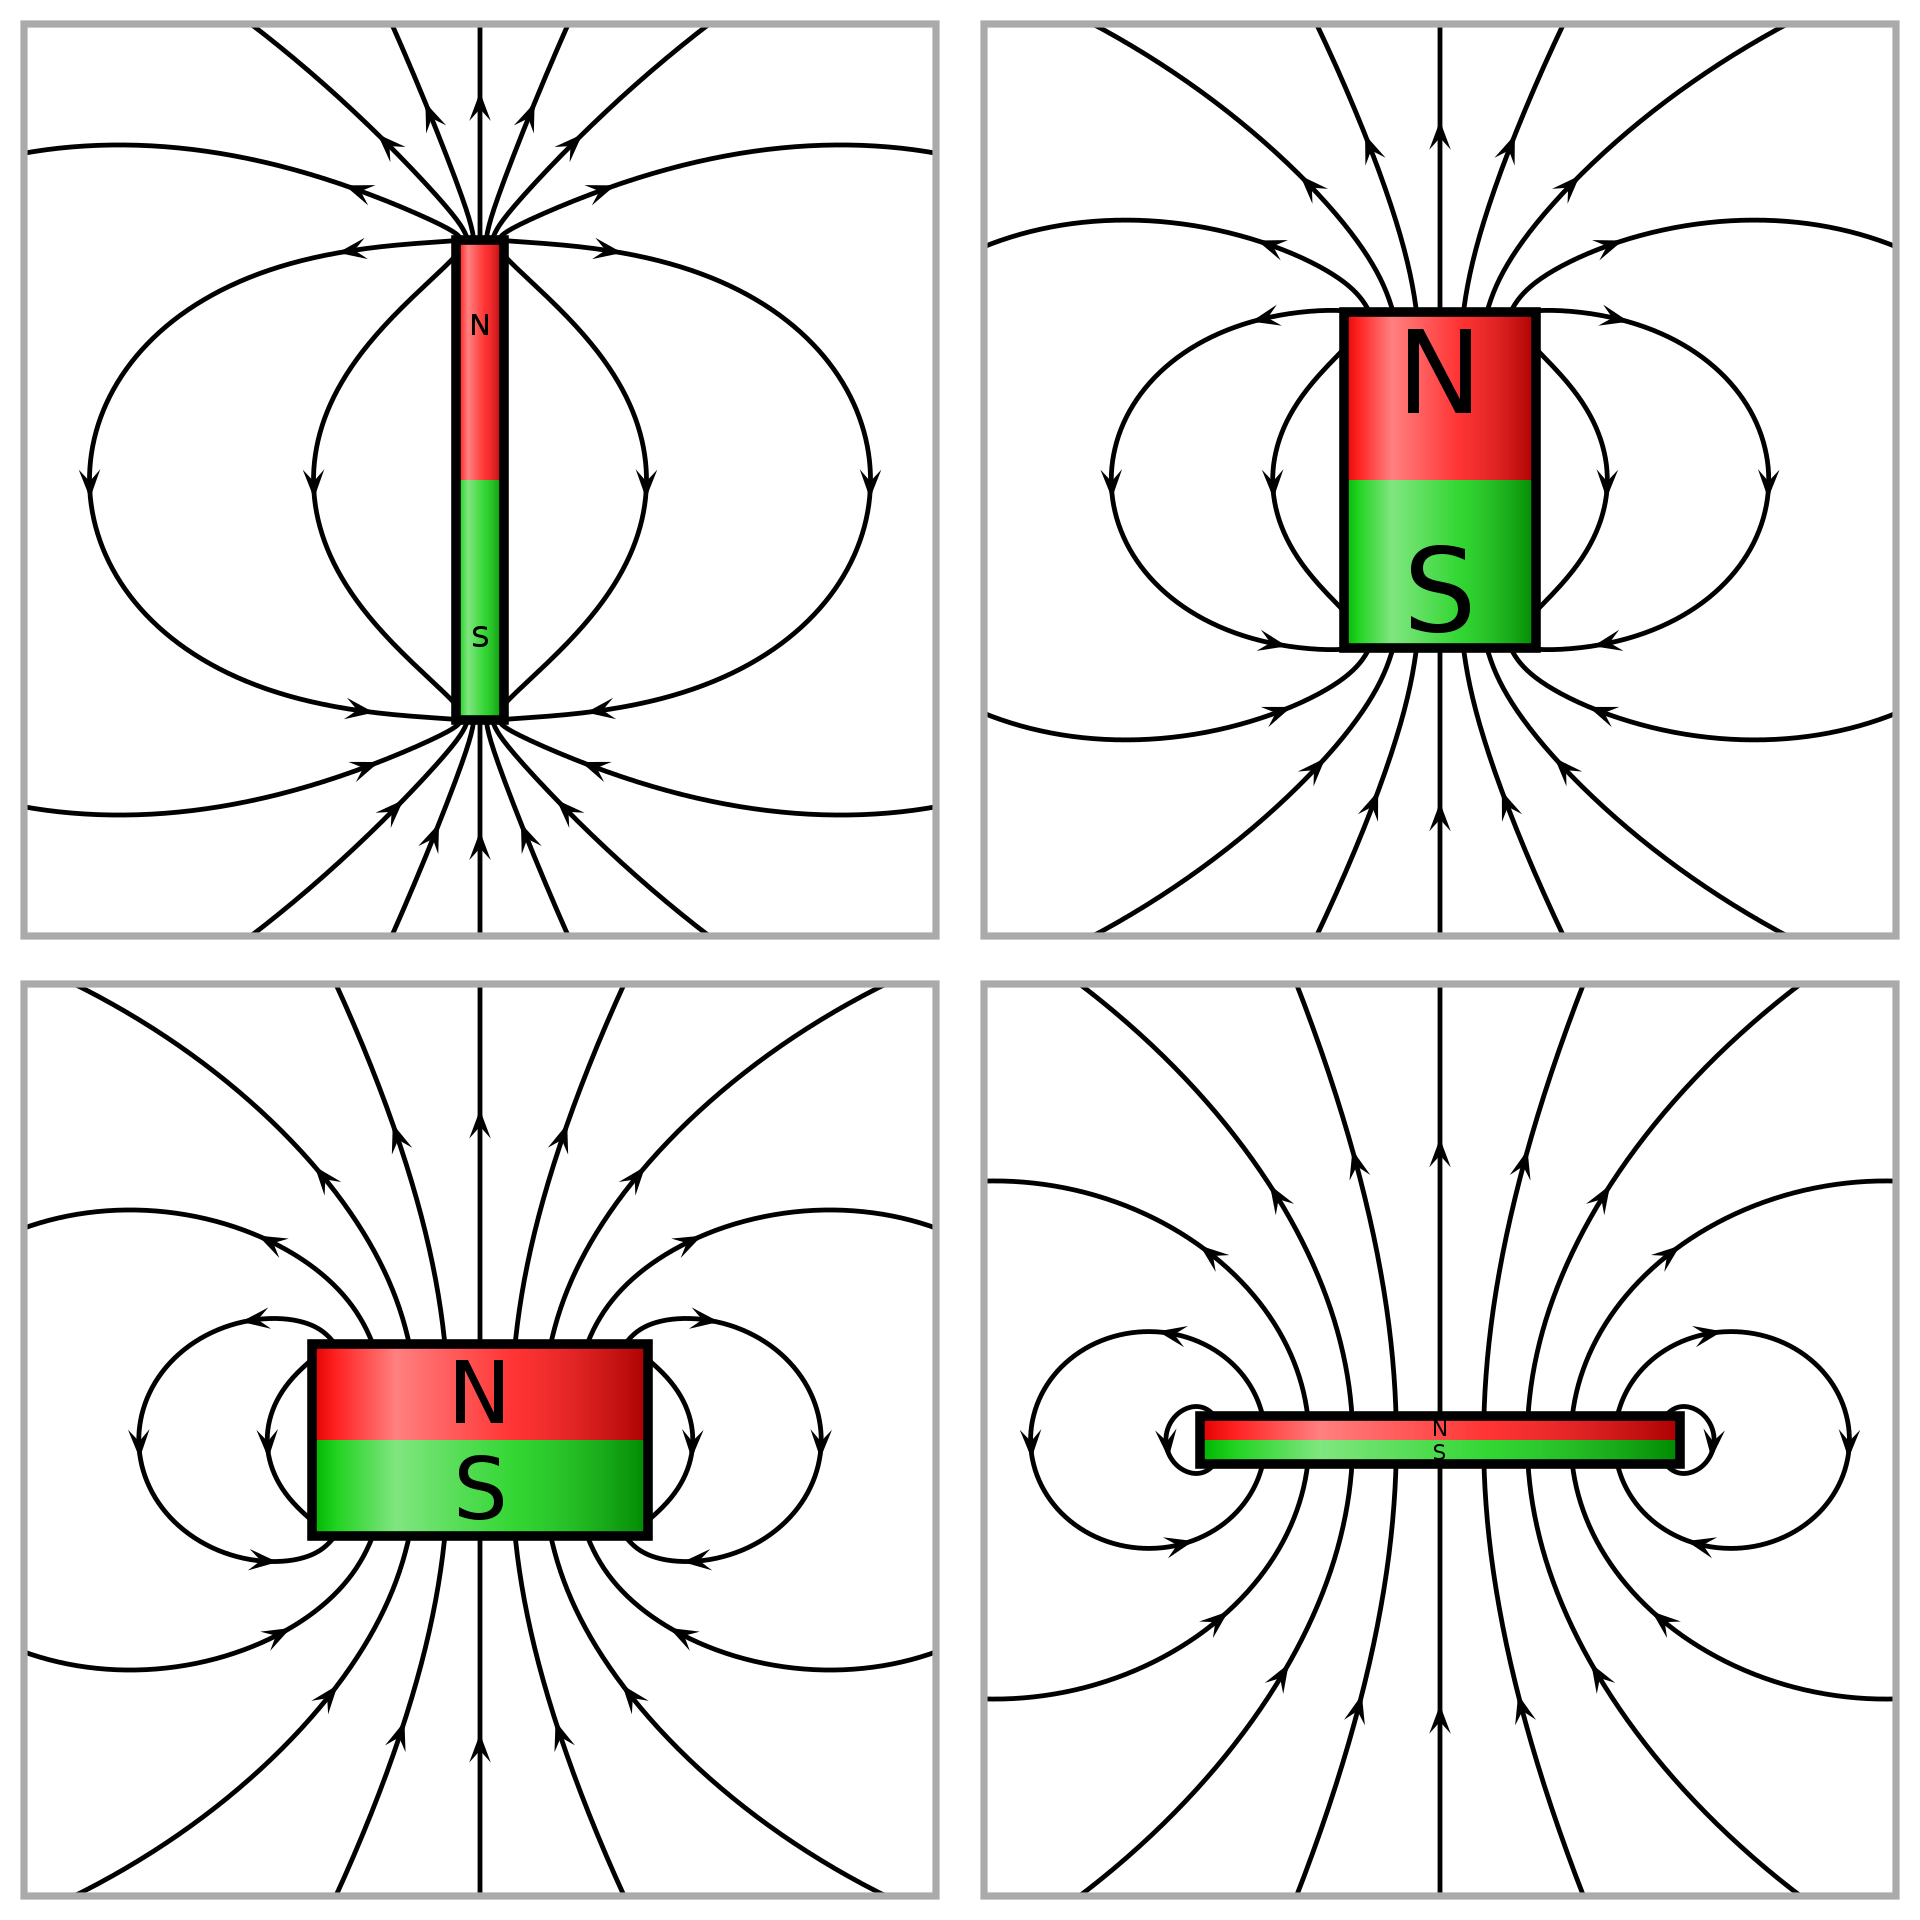
\includegraphics[scale=0.075]{assets/magnets.png}

Since magnetic fields exert force on currents/moving charges, it is necessary to describe the force associated with them: the interaction.

The force experienced by moving charges or currents in magnetic fields are described by the following relations.

\[\vec{F} = q\vec{v}\times\vec{B} \qquad \vec{F} = I\vec{l}\times\vec{B} \qquad \vec{F} = q(\vec{E} + \vec{v}\times\vec{B})\]

On the left is the force exerted on moving charges -- notice how force is only exerted when the charge is moving with non-zero velocity. The middle describes the force exerted on a current. It might be easier to think of the direction of the force with the direction of the current instead of the length of the current. The right presents an equation for the electromagnetic forces exerted on a point charge.

\[\mathbf{F} = q\mathbf{v}\mathbf{B}\sin\theta \qquad \mathbf{F} = I\mathbf{l}\mathbf{B}\sin\theta\]

It is worth noting that the cross product is hard to calculate, and most of times we use the trig equivalent of the expression for calculations, as shown above.

\hfil 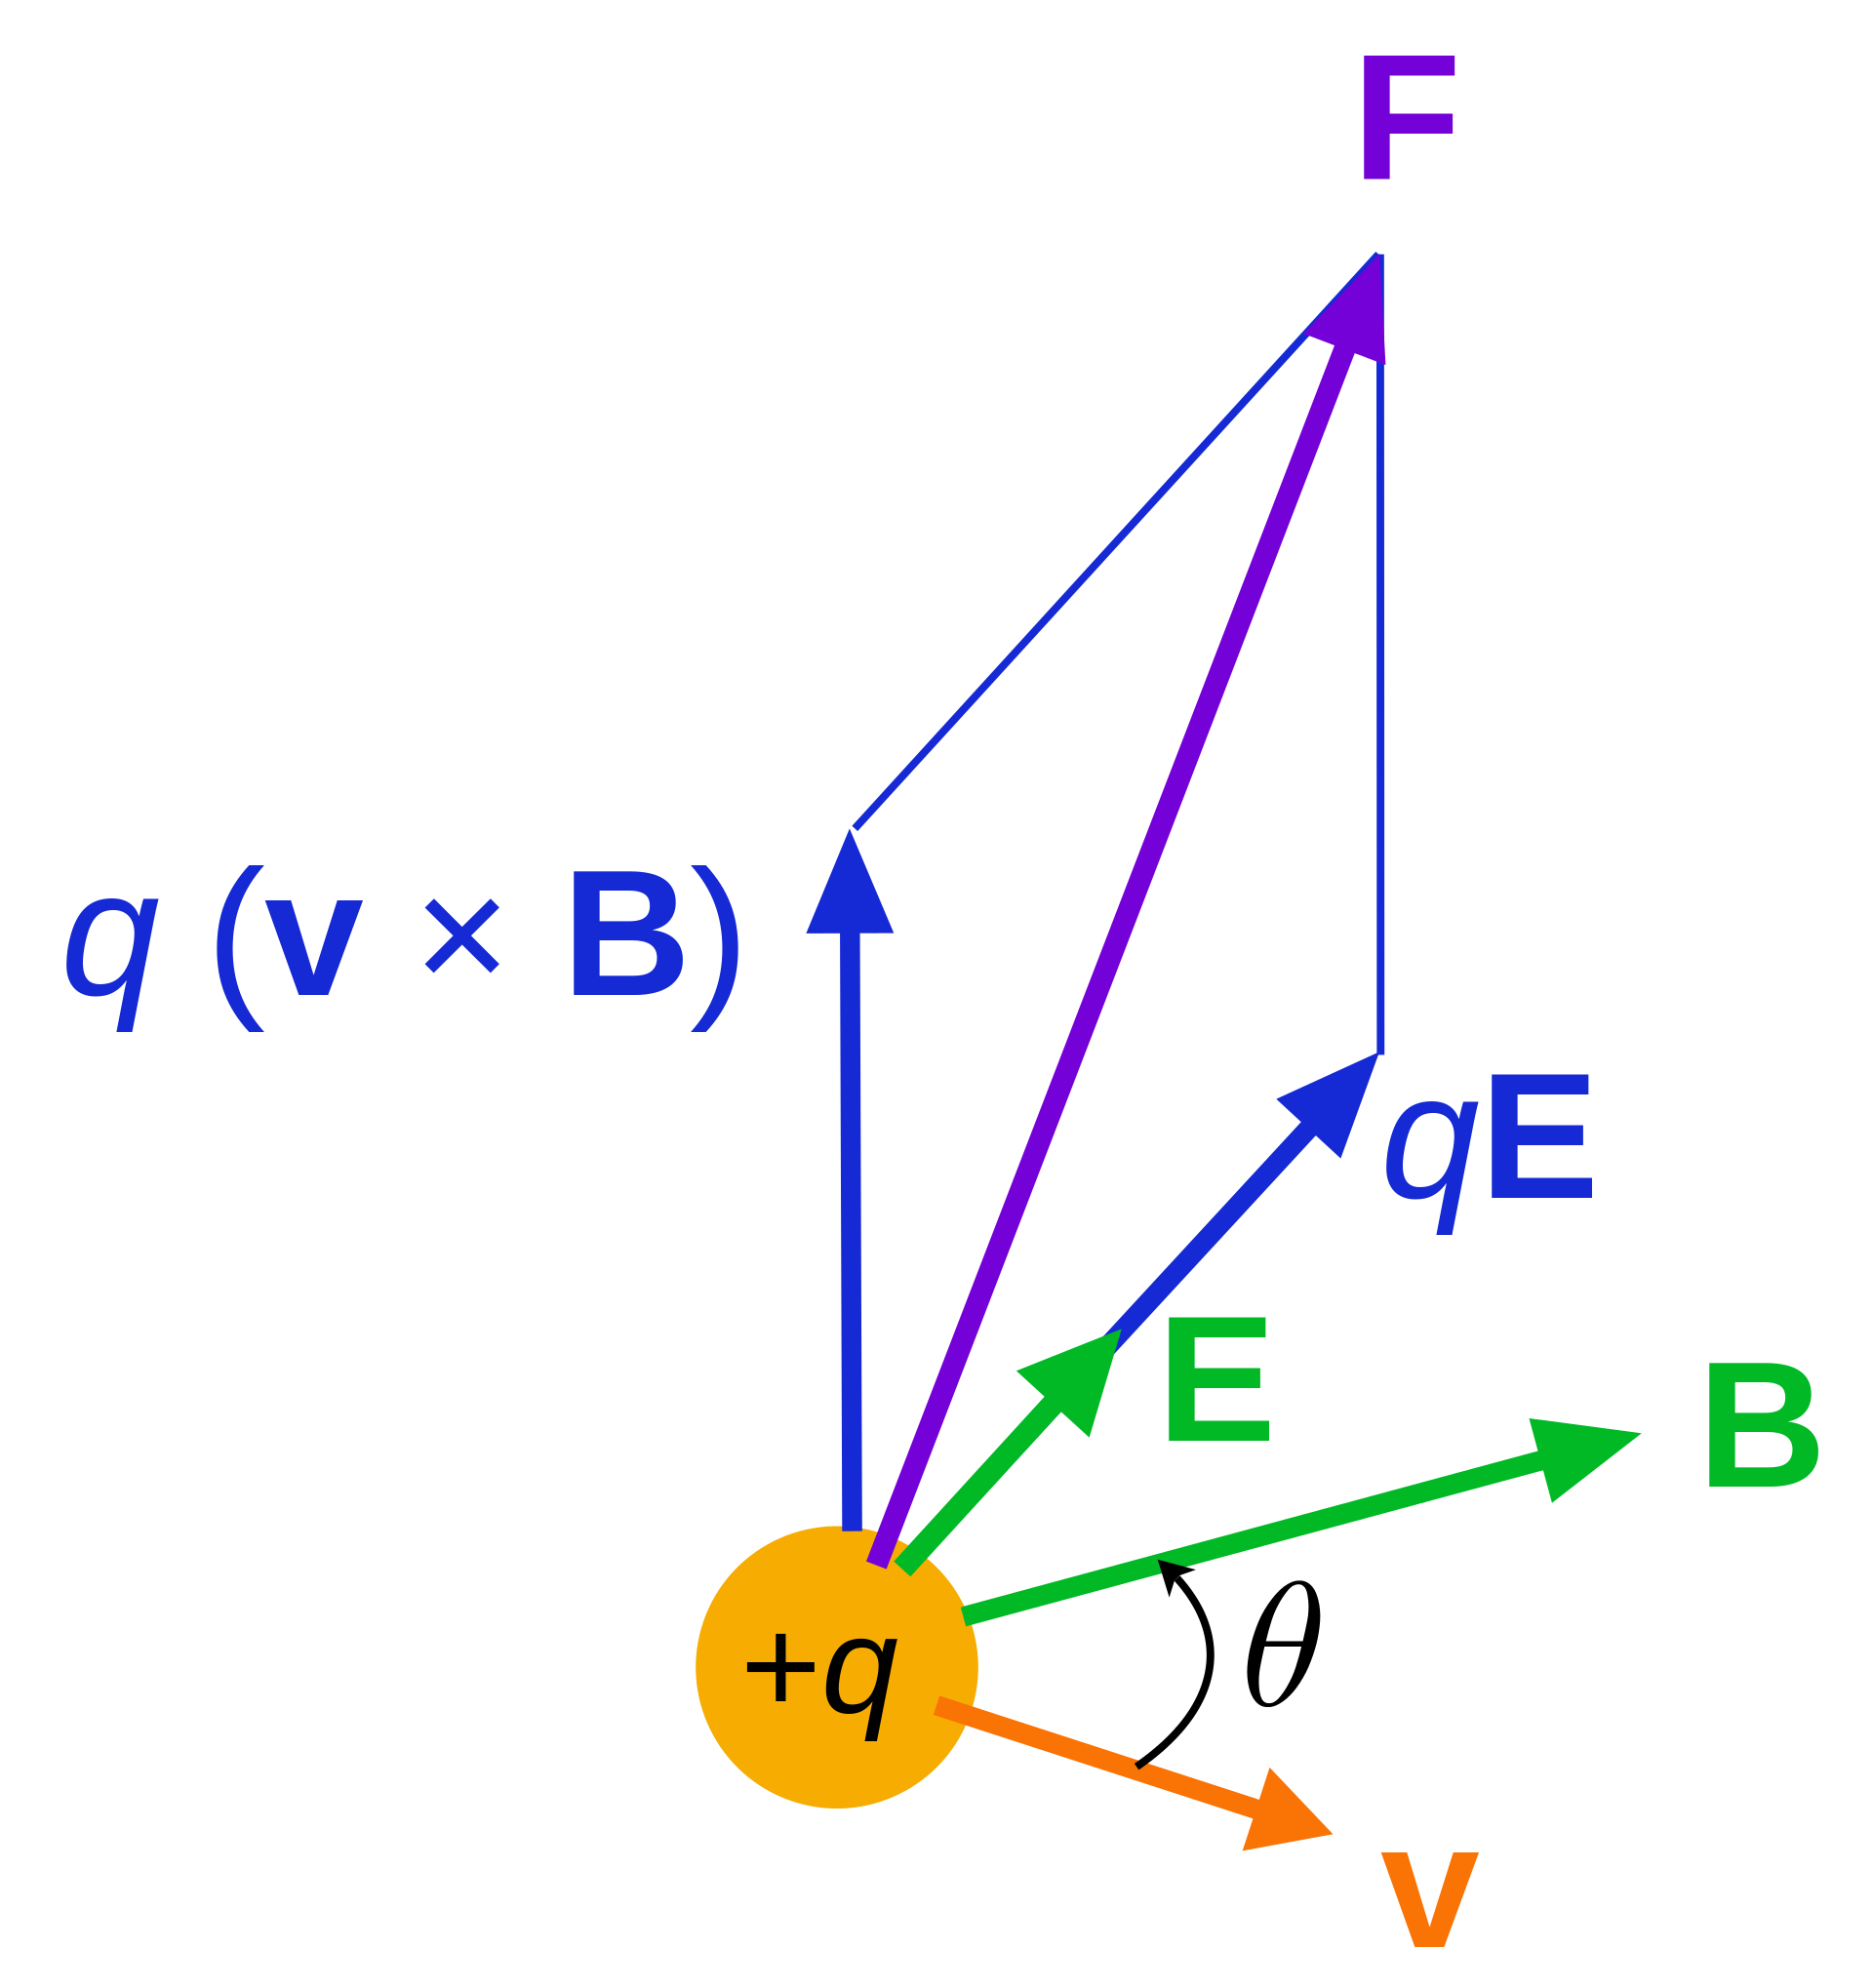
\includegraphics[scale=0.075]{assets/lorentz-force.png}

We can use the right hand rule for thinking about the direction of the cross product. This also implies that the force is always perpendicular to the direction of the magnetic field and the velocity vector. The force is also perpendicular to the magnetic field and the current passthrough. 

\subsection{Applications}



\section[Laws of Magnetism]{Gauss's Law for Magnetism \& Ampere's Law}

Similar to the electric field, Gauss came up with another law for magnetic fields.

\[\oiint_S B\cdot\dif S = 0\]

To understand why this is true, consider the following current loop (or any magnet)

\hfil 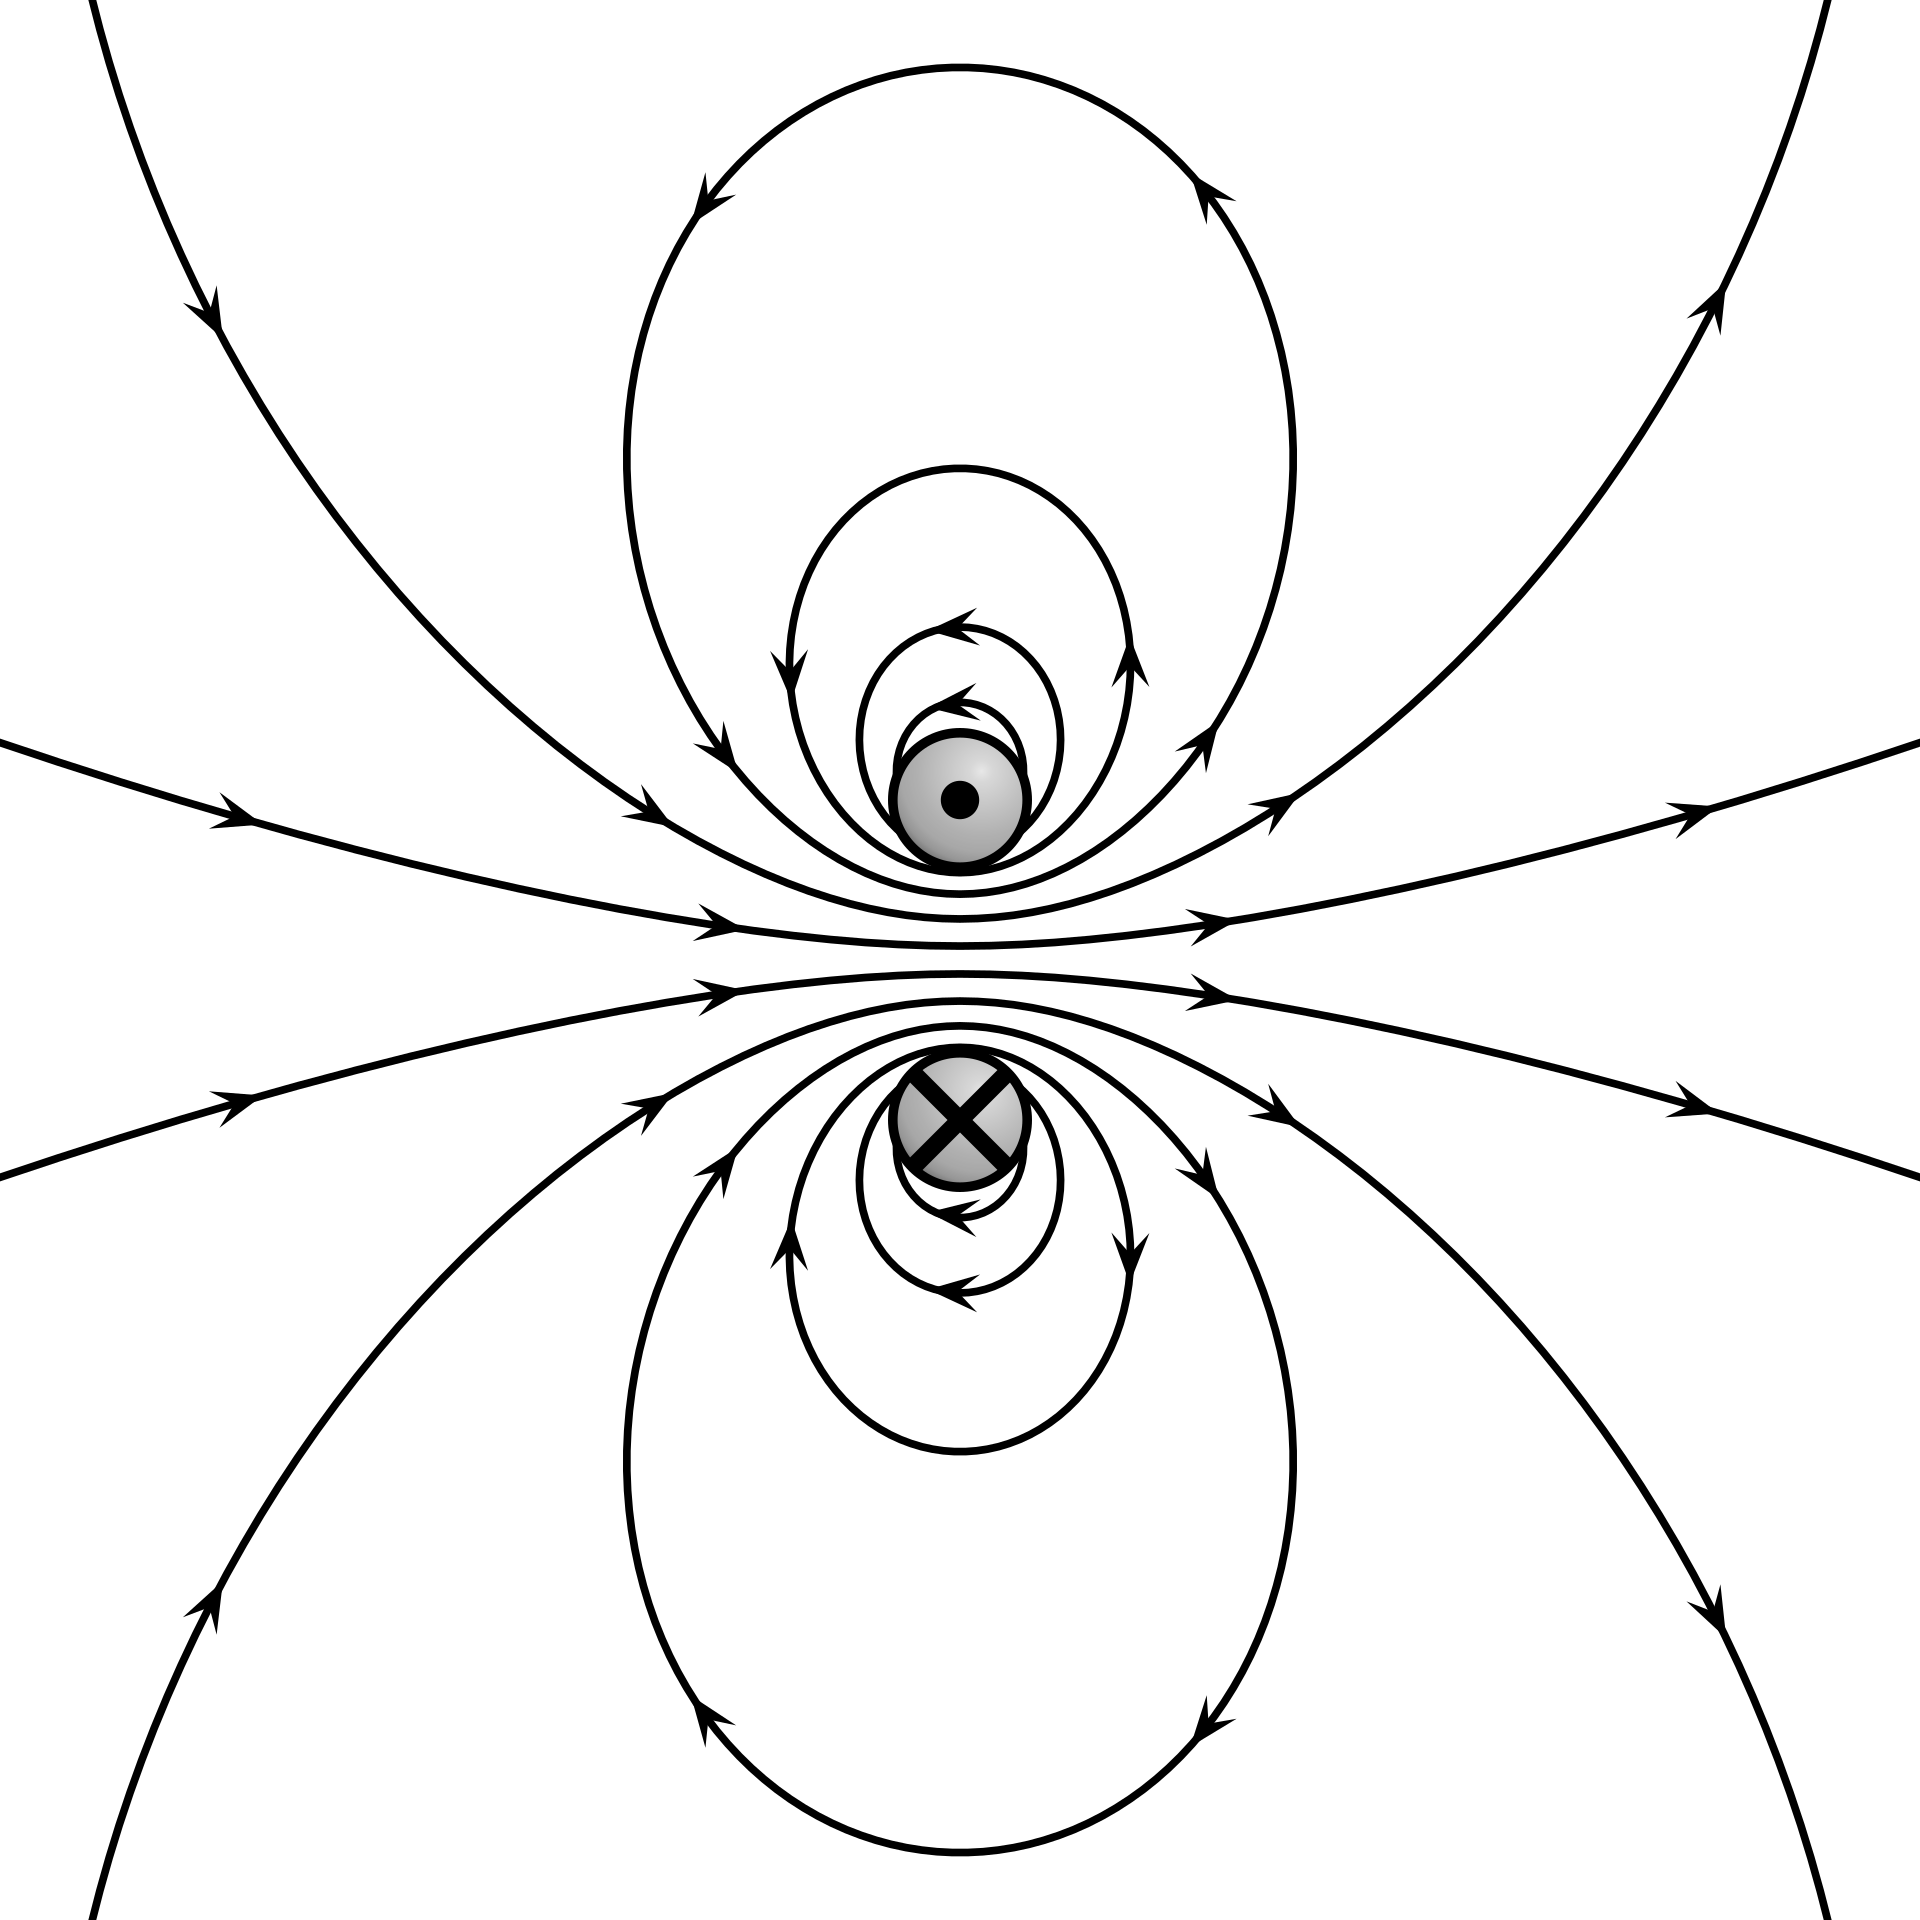
\includegraphics[scale=0.05]{assets/mag-i-loop.png}

When we form a close surface and trace the field lines of the magnetic field at any point, we discover that whatever goes out also comes in (in other words, there are no starts or ends for magnetic field lines, they are in the form of loops), making the net magnetic flux out of any closed surface 0 -- intuitively, for every line out, it has to come back in. This relationship is described by \textbf{Gauss's Law for Magnetism}, shown above.

Then there is \textbf{Ampere's Law}:

\[\oint_C B \cdot \,\dif l = \mu_0 I_{\mathrm{enc}}\]

\hfil in the form that we are concerned with,

where $B$ is the magnetic field, $C$ is the closed path for which we are integrating along, $\mu_0$ is the \textbf{Vacuum Permeability} (value shown below), and $I_{\mathrm{enc}}$ is the amount of current passing through the surface enclosed by path $C$.

\[\mu_0 = \SI{1.25663706212(19)e-6}{\henry\per\meter}\]

This is similar to Gauss's Law for measuring electric flux out of some gaussian surface. Ampere's Law, combined with Gauss's Law for Magnetism will be helpful in finding the magnetic field of different currents.

\section{Applications of Ampere's Law}

We list a few different scenarios where we can derive the expression for magnetic field utilizing the two rules are described above.

\subsection{Single Long Straight Wire/Current}

\hfil 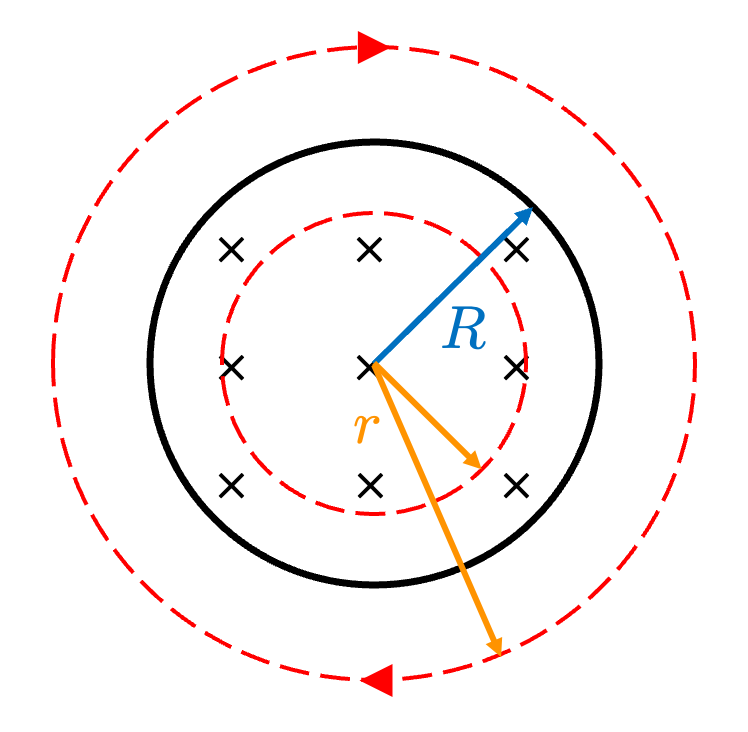
\includegraphics[scale=0.4]{assets/amp-law-single-wire.png}

There are actually two regions that we can consider for a long straight wire: regions inside the wire and regions outside the wire. Let us assume that the wire has a radiums of $R$ and represent our magnetic field at some radius $r$ as $B$.

First for $r > R$:

\dots

Now, $r < R$:

\dots


\subsection{Sheet of Wires/Currents}

\hfil 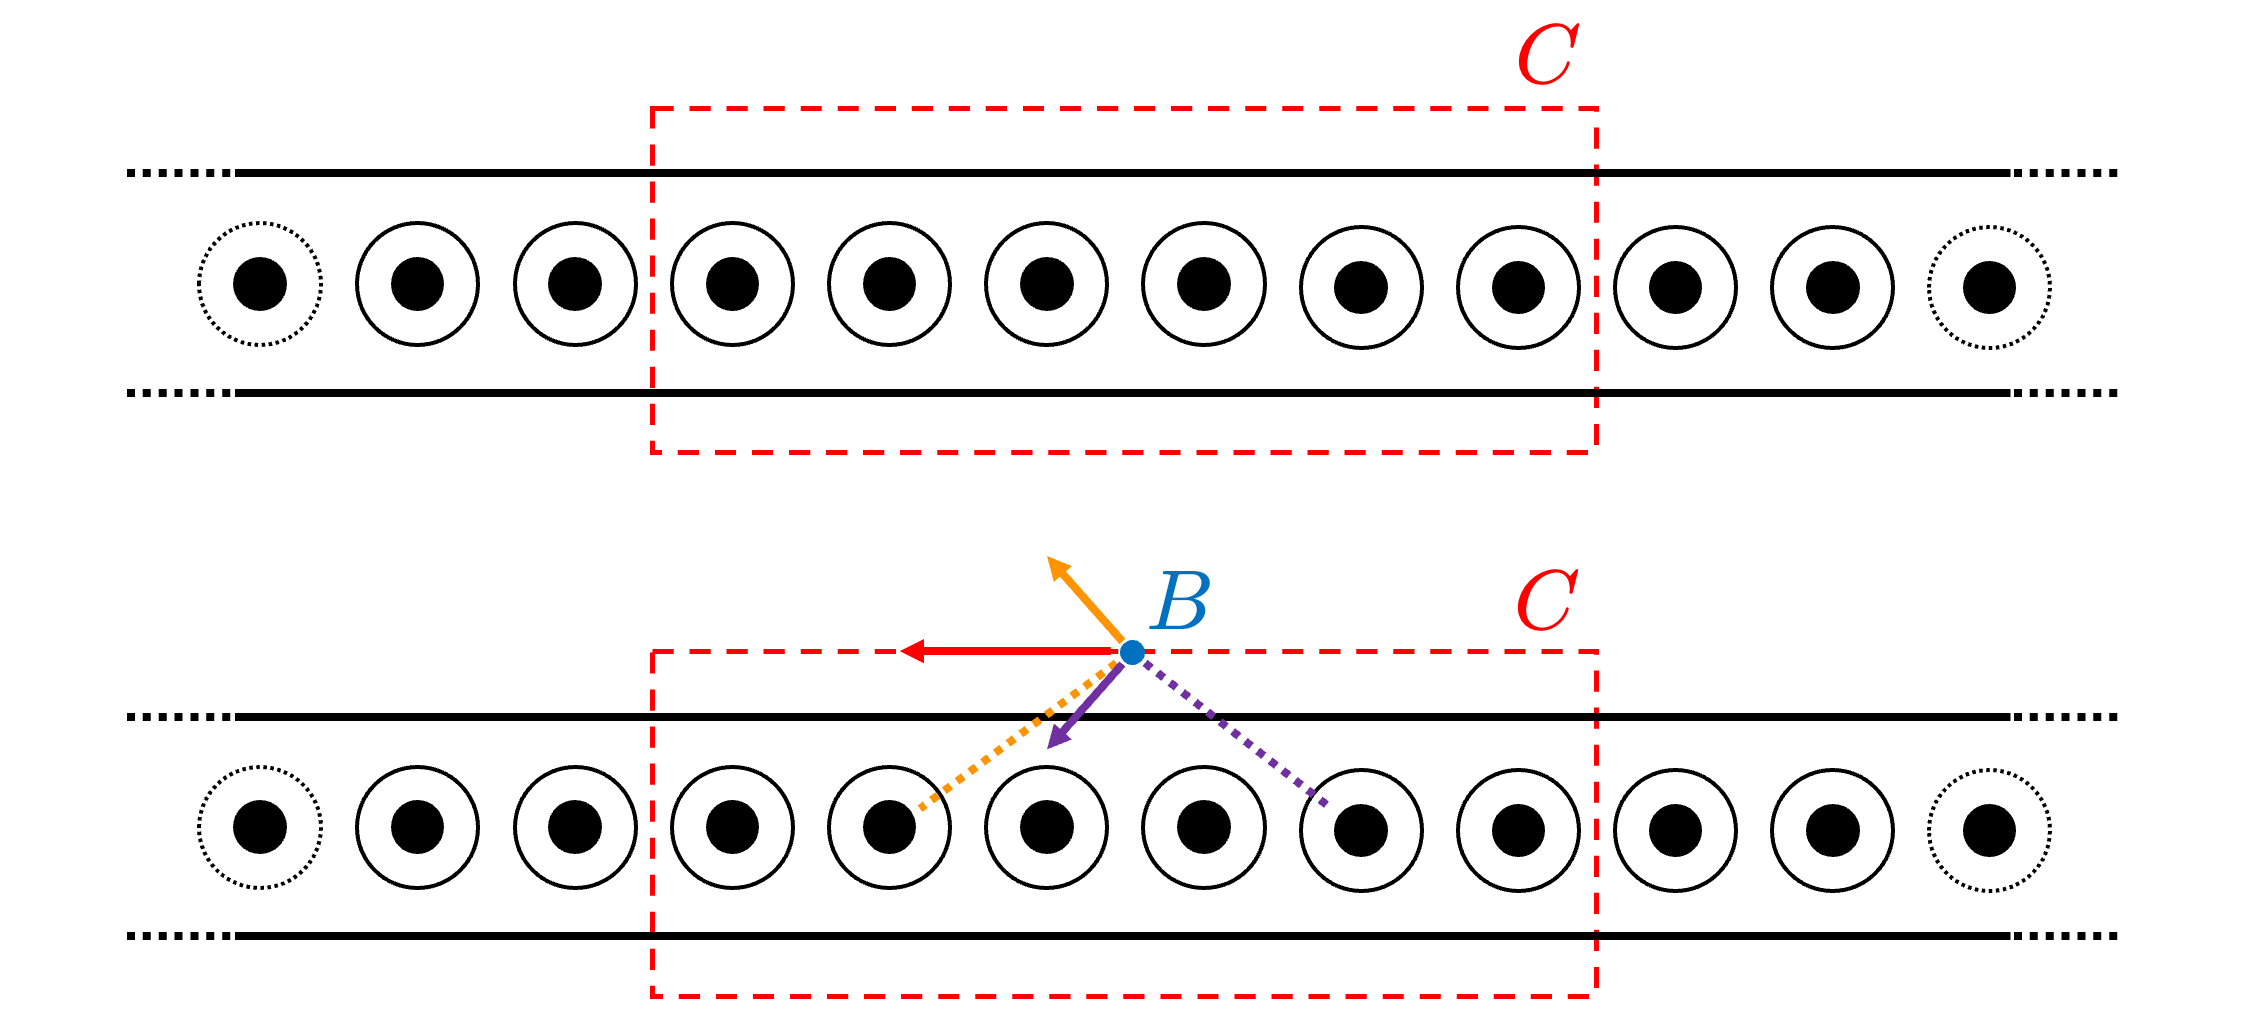
\includegraphics[scale=0.15]{assets/amp-law-current-sheet.png}

Now that we have considered a single straight wire, we can also consider a sheet of current/wires and the magnetic field that this creates.

\subsection{Solenoids}

\hfil 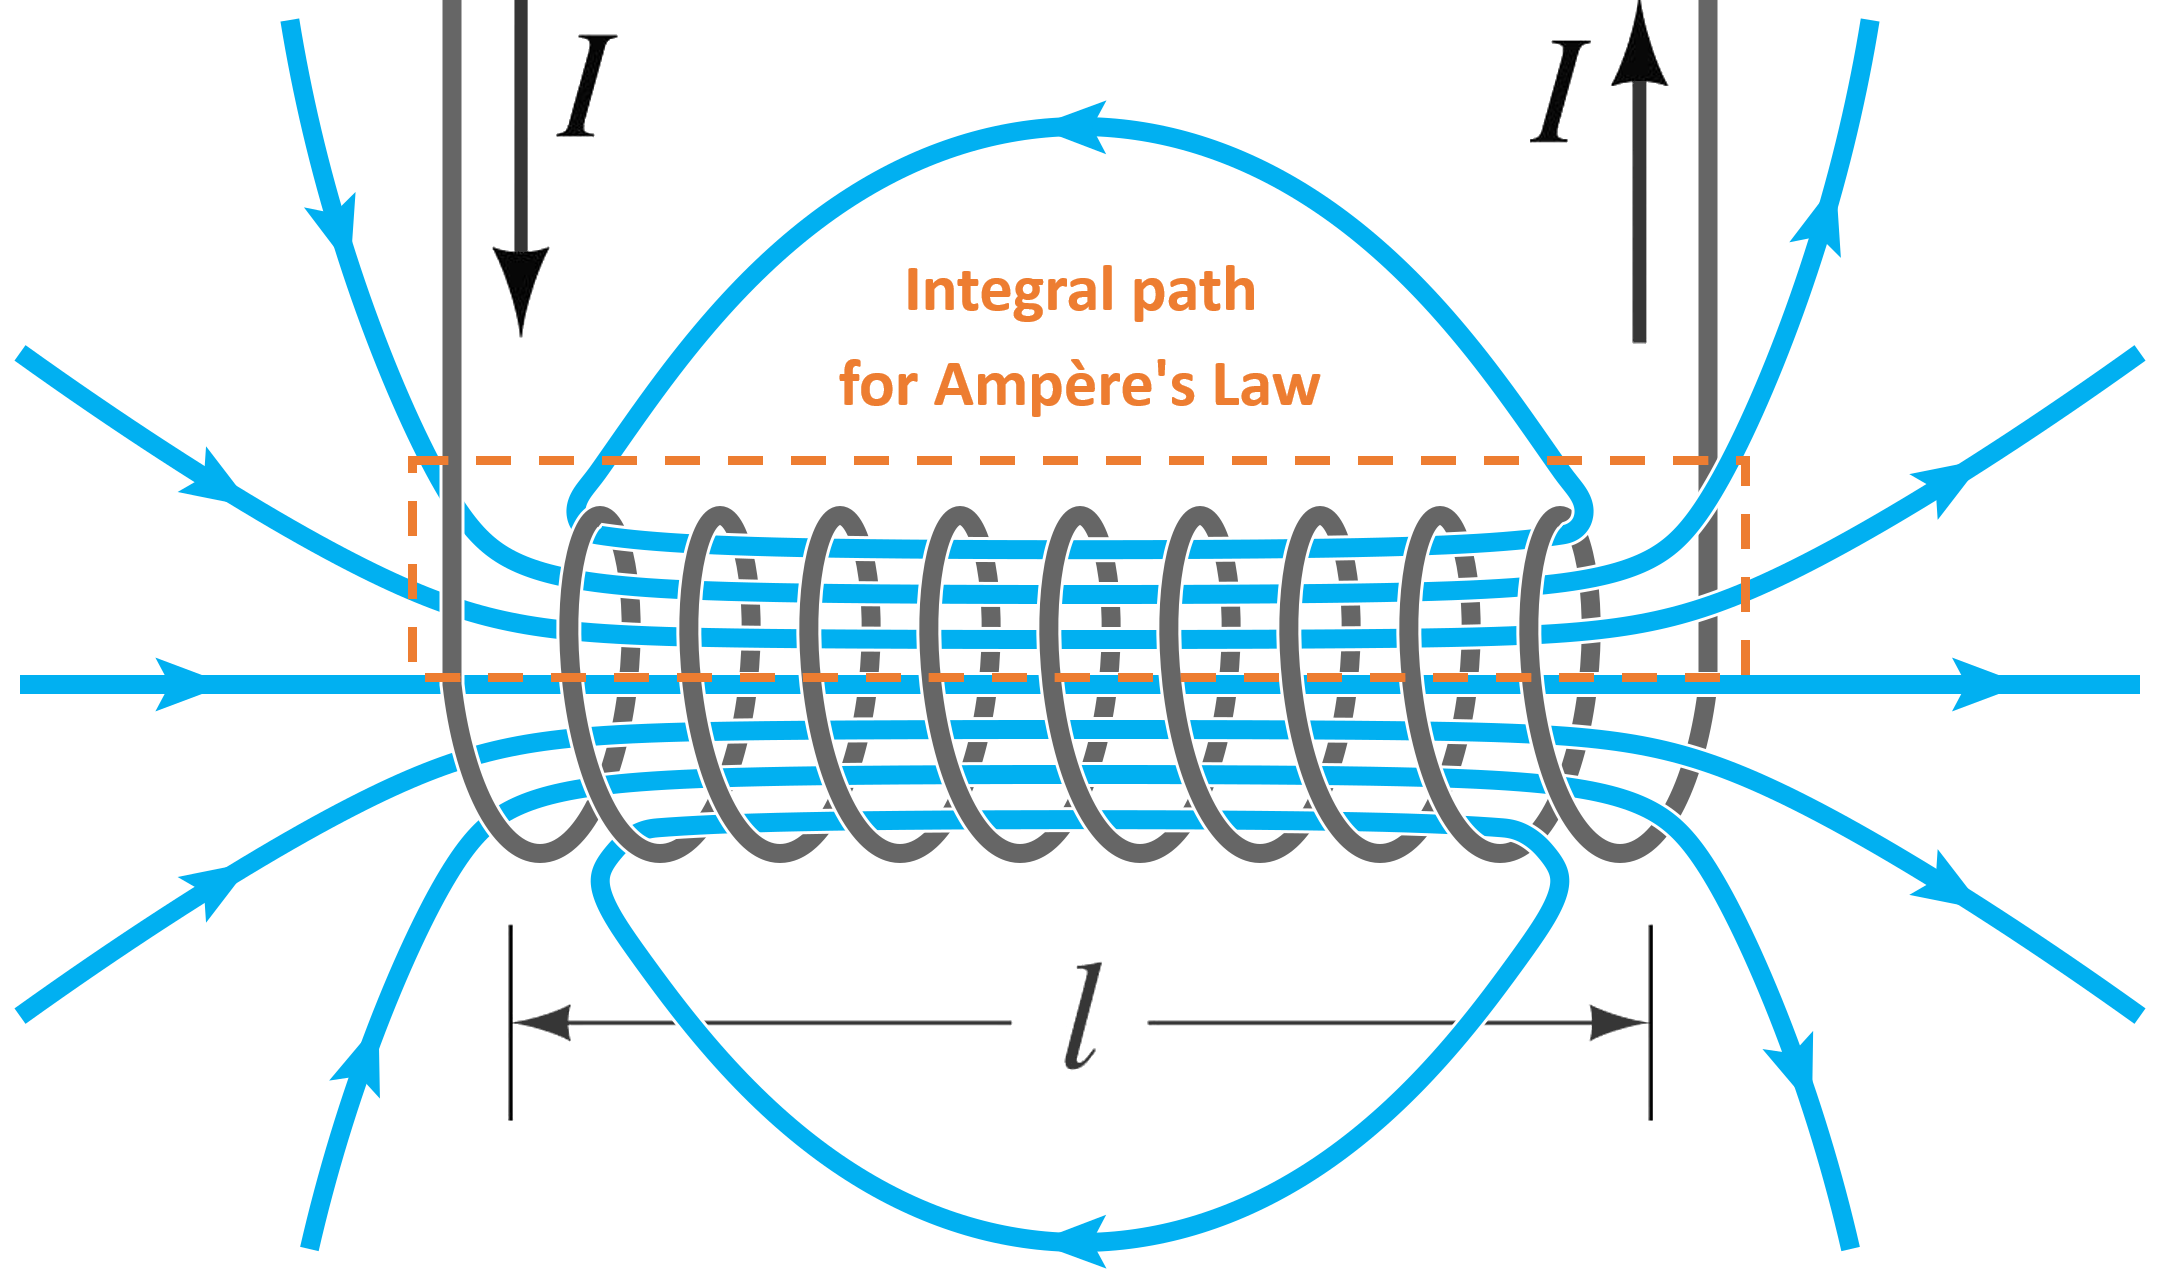
\includegraphics[scale=0.1]{assets/amp-law-solenoid.png}

For this case we will consider idealized solenoids where we consider the magnetic field outside the solenoid to be 0.

\section{Biot-Savart Law}

\subsection{Law}


\subsection{Moving Charges}


\section{Derivation for Field of Currents}

	\chapter{Inductance}



	\appendix

	\chapter{Resources \& References}

Physics Vol. 2 -- Halliday, Resnick, Krane

\textbf{ISBN-13:} 978-0471401940 \textbf{ISBN-10:} 0471401943

\href{https://www.amazon.com/Physics-2-David-Halliday/dp/0471401943/}{Amazon}

\bigskip

Barron's AP Physics C 

\textbf{ISBN-13:} 978-1438012858 \textbf{ISBN-10:} 1438012853

\href{https://www.amazon.com/AP-Physics-Practice-Tests-Barrons/dp/1438012853/}{Amazon}

\bigskip

Electromagnetism Articles on Wikipedia:

\href{https://en.wikipedia.org/wiki/Electromagnetism}{https://en.wikipedia.org/wiki/Electromagnetism}

\bigskip

HyperPhysics:

\href{http://hyperphysics.phy-astr.gsu.edu/}{http://hyperphysics.phy-astr.gsu.edu/}

\bigskip

Questions on Stack Exchange:

\href{https://stackexchange.com/}{https://stackexchange.com/}
\end{document}